%~ \documentclass[letterpaper,times,draft]{sae}
\documentclass[letterpaper,times]{sae}

\usepackage[svgnames]{xcolor}
\definecolor{SAEblue}{RGB}{1,160,233}
%\raggedright

\usepackage[justification=justified, singlelinecheck=false]{caption}  % ,figurename=Fig.,labelfont={it}
\DeclareCaptionFont{eightpt}{\fontsize{8pt}{11pt}\selectfont #1}
\captionsetup{font={eightpt,color=SAEblue}}

\usepackage{lineno}
\usepackage[utf8]{inputenc}

\usepackage{array}% http://ctan.org/pkg/array (also necessary for width calculations (for vert. lines)))
\newcolumntype{L}[1]{>{\raggedright\let\newline\\\arraybackslash\hspace{0pt}}p{#1}}
\newcolumntype{C}[1]{>{\centering\let\newline\\\arraybackslash\hspace{0pt}}p{#1}}
\newcolumntype{R}[1]{>{\raggedleft\let\newline\\\arraybackslash\hspace{0pt}}p{#1}}

\usepackage{graphicx}
\usepackage{multirow}
\usepackage{amsmath}
\usepackage{cite} % Sort and compress consecutive numeric citations (e.g., [1--4])

% Charge le module graphique tikz
\usepackage{tikz}
\usepackage{pgfplots}
\usetikzlibrary{backgrounds}
\usetikzlibrary{shapes,decorations,shadows,arrows,calc}
\usetikzlibrary{decorations.markings}

\newcommand{\ignore}[1]{}
\newcommand{\todo}[1]{\textcolor{red}{TODO: {#1}}}
\newcommand{\todr}[1]{\textcolor{purple}{CAN CUT: {#1}}}
\newcommand{\todm}[1]{\textcolor{green}{MOVE: {#1}}}
\newcommand{\case}[1]{\mbox{\textit{#1}}}
\newcommand{\textss}[1]{\textsuperscript{#1}}
\renewcommand{\deg}{$^\circ$}


\newcommand{\Figref}[1]{Figure \ref{#1}}
\newcommand{\Figrefs}[2]{Figures \ref{#1} and \ref{#2}}
\newcommand{\Figrefsto}[2]{Figures \ref{#1} to \ref{#2}}
\newcommand{\Tabref}[1]{Table \ref{#1}}
\newcommand*{\dt}[1]{%
\accentset{\mbox{\large\bfseries .}}{#1}}
\usepackage{nameref}
\usepackage{booktabs}

% Define "struts" as suggested by Claudio Beccari in
% a piece in TeX and TUG News, Vol. 2, 1993.
\newcommand\Tstrut{\rule{0pt}{4.6ex}}       % "top" strut
\newcommand\Bstrut{\rule[-0.9ex]{0pt}{0pt}} % "bottom" strut
\newcommand{\TBstrut}{\Tstrut\Bstrut} % top&bottom struts

%%% the following hides the section number while keeping their numbering for proper referencing in toc and \ref
\makeatletter
\def\@seccntformat#1{%
  \expandafter\csname c@#1\endcsname\c@section
  }
\makeatother

\usepackage{subfigure}
\usepackage{multimedia}

\DeclareMathOperator{\sign}{sign}
\newcommand{\quotes}[1]{``#1''}


\PaperTitle{CHAMPS Contribution to the Third AIAA Ice Prediction Workshop}
\usepackage{calc} % to get proper table widths (subtracting colsep and black lines width

\makeatletter 
\renewcommand\@biblabel[1]{#1. } 
\makeatother

\AddAuthor{Karim Zayni}{Department of Mechanical Engineering, Polytechnique Montr\'{e}al, Montr\'{e}al, Canada}
\AddAuthor{Maxime Blanchet}{Department of Mechanical Engineering, Polytechnique Montr\'{e}al, Montr\'{e}al, Canada}
\AddAuthor{Eric Laurendeau}{Department of Mechanical Engineering, Polytechnique Montr\'{e}al, Montr\'{e}al, Canada}
\PaperNumber{2027-XX-XXXX}
\SAECopyright{2027}



\begin{document}
\maketitle

% ============================================================
% ABSTRACT
% ============================================================

\begin{abstract}

This paper presents the contribution of Polytechnique Montr\'{e}al to the Third AIAA Ice Prediction Workshop (IPW3) using the in-house \textsc{CHAMPS} multiphysics software. The study provides a component-wise verification and validation of the numerical icing chain for the three-dimensional NACA~0012 and ONERA~M6 configurations, including aerodynamic flow, droplet impingement, thermodynamics, and ice accretion. Predictions are evaluated across the prescribed workshop grid hierarchies and droplet-size discretizations, with complementary Eulerian and Lagrangian droplet calculations providing an independent verification of impingement. The results show that convergence of integrated quantities does not necessarily imply convergence of local distributions: collected-water mass exhibits relatively limited sensitivity to droplet discretization while impingement limits remain more strongly affected. Aerodynamic and impingement predictions are generally consistent across grid levels and with the IPW3 code-to-code envelope. Single-layer ice shapes exhibit limited spatial sensitivity and generally remain within the experimental envelopes. Multilayer simulations produce more complex three-dimensional morphologies but do not necessarily improve agreement with experiment. The component-wise analysis provides a systematic verification and validation of \textsc{CHAMPS} under the common IPW3 framework and identifies droplet discretization, thermodynamics, surface roughness, and geometry evolution as important sensitivities in the coupled icing prediction.

\end{abstract}

% ============================================================
% INTRODUCTION
% ============================================================

\section{Introduction}

Aircraft ice accretion is a strongly coupled multiphysics phenomenon involving aerodynamic flow, supercooled water-droplet impingement, surface thermodynamics, and progressive evolution of the iced geometry. Ice contamination can substantially modify the effective shape of lifting surfaces and degrade aerodynamic performance \cite{CAO2018353,broeren2011aerodynamic,KIND1998257}. Reliable numerical icing tools therefore require accurate prediction not only of the final ice geometry but also of the individual physical components contributing to the accretion process.

Verification and validation are particularly important for numerical icing because numerical and modeling errors can propagate through successive components of the icing chain. Agreement in the final ice shape may result from compensating errors between these components. Evaluating the aerodynamic, droplet-impingement, and thermodynamic predictions separately therefore helps identify the source of differences observed in the final ice prediction. Consequently, aerodynamic quantities, droplet collection, thermodynamic response, and ice geometry should be examined individually in addition to the final accretion \cite{wright2008manual,bourgault1999eulerian}.

The AIAA Ice Prediction Workshops provide standardized configurations, computational grids, experimental measurements, and code-to-code comparisons for systematic verification and validation of numerical icing tools \cite{laurendeau2022summary,laurendeau2024summary}. The Third AIAA Ice Prediction Workshop (IPW3) extends this effort through three-dimensional configurations and common grid hierarchies that enable consistent evaluation of spatial discretization and modeling sensitivities.

The present work summarizes the contribution of Polytechnique Montr\'{e}al to IPW3 using the in-house \textsc{CHAMPS} multiphysics solver \cite{champsArticle}. Two three-dimensional configurations are considered: the NACA~0012 and the swept ONERA~M6 wing. The significant contribution of this work is a component-wise verification and validation of the complete \textsc{CHAMPS} icing chain under the common IPW3 framework. Spatial refinement, droplet-size discretization, Eulerian and Lagrangian impingement formulations, thermodynamics, and single- and multilayer geometry evolution are examined to identify the numerical and modeling sensitivities influencing the final ice prediction.

% ============================================================
% METHODOLOGY
% ============================================================

\section{Methodology}

The simulations are performed using the unstructured finite-volume \textsc{CHAMPS} multiphysics solver developed at Polytechnique Montr\'{e}al \cite{champsArticle}. The overall numerical icing sequence is illustrated in Fig.~\ref{fig:icingFramework}. The aerodynamic flow is first computed, followed by droplet impingement, surface thermodynamics, and ice growth. For multilayer simulations, the iced geometry is subsequently remeshed and the sequence is repeated.

\begin{figure}[htb]
    \centering
    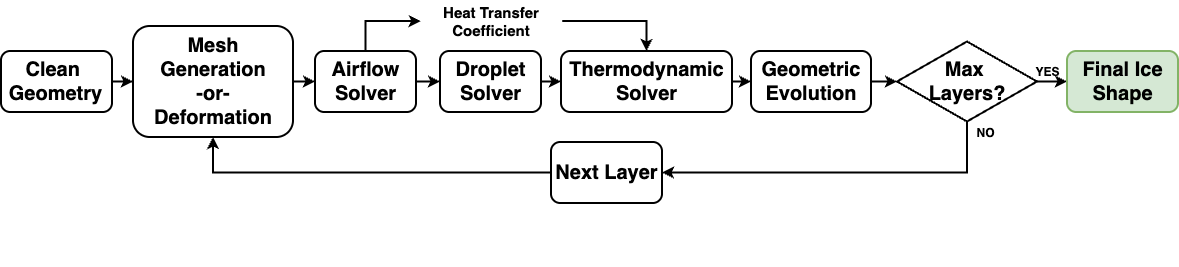
\includegraphics[width=0.88\linewidth]{FIGURES/LS_FRAMEWORK/icingFramework.png}
    \caption{Multiphysics ice-accretion framework implemented in \textsc{CHAMPS}.}
    \label{fig:icingFramework}
\end{figure}

The aerodynamic calculations use the compressible Reynolds-averaged Navier--Stokes equations with the Spalart--Allmaras turbulence model \cite{spalart1992one} and Aupoix roughness correction \cite{aupoix2003roughness}. Roe convective fluxes \cite{roe1981approximate} and a Venkatakrishnan limiter \cite{venkatakrishnan1995convergence} are employed.

Supercooled droplets are modeled using an Eulerian formulation based on the continuum representation of the dispersed phase \cite{bourgault1999eulerian}. Complementary Lagrangian calculations are performed to independently verify the predicted collection efficiency and collected-water mass. The use of multiple discrete droplet diameters follows the conventional representation of droplet-size distributions employed in aircraft icing calculations \cite{wright2008manual}.

Surface thermodynamics are evaluated using an iterative formulation based on the classical Messinger surface energy balance \cite{messinger1953equilibrium}. Single-layer ice geometries are generated using an algebraic surface-displacement approach, while multilayer calculations use the continuous level-set methodology developed within \textsc{CHAMPS}. Level-set methods provide an implicit representation of evolving interfaces through the zero contour of a scalar field \cite{OSHER198812,OSHER2004}. Following each accretion layer, the interface is extracted using \textsc{MMG} \cite{DAPOGNY2014358} and the aerodynamic domain is regenerated using automated \textsc{Pointwise} procedures.

The IPW3 comparisons are performed over the prescribed grid hierarchies and droplet-size distributions. Quantities considered include integrated aerodynamic coefficients, local pressure and collection-efficiency distributions, collected-water and ice masses, and experimental ice geometries. This component-wise procedure is used to distinguish numerical convergence of integrated quantities from convergence of local distributions and agreement with experimental measurements.

% ============================================================
% PRELIMINARY RESULTS
% ============================================================

\section{Preliminary Results}

% ------------------------------------------------------------
% NACA0012
% ------------------------------------------------------------

\subsection{NACA~0012}

The NACA~0012 grid hierarchy ranges from approximately $5.9$ million cells on Level~4 to $59.9$ million cells on Level~1. Aerodynamic predictions remain well clustered over the finer grids. The surface-pressure coefficient distributions are well positioned within the participant envelope and closely follow the experimental measurements, as illustrated in Fig.~\ref{fig:nacaAero}.

\begin{figure}[htb]
    \centering
    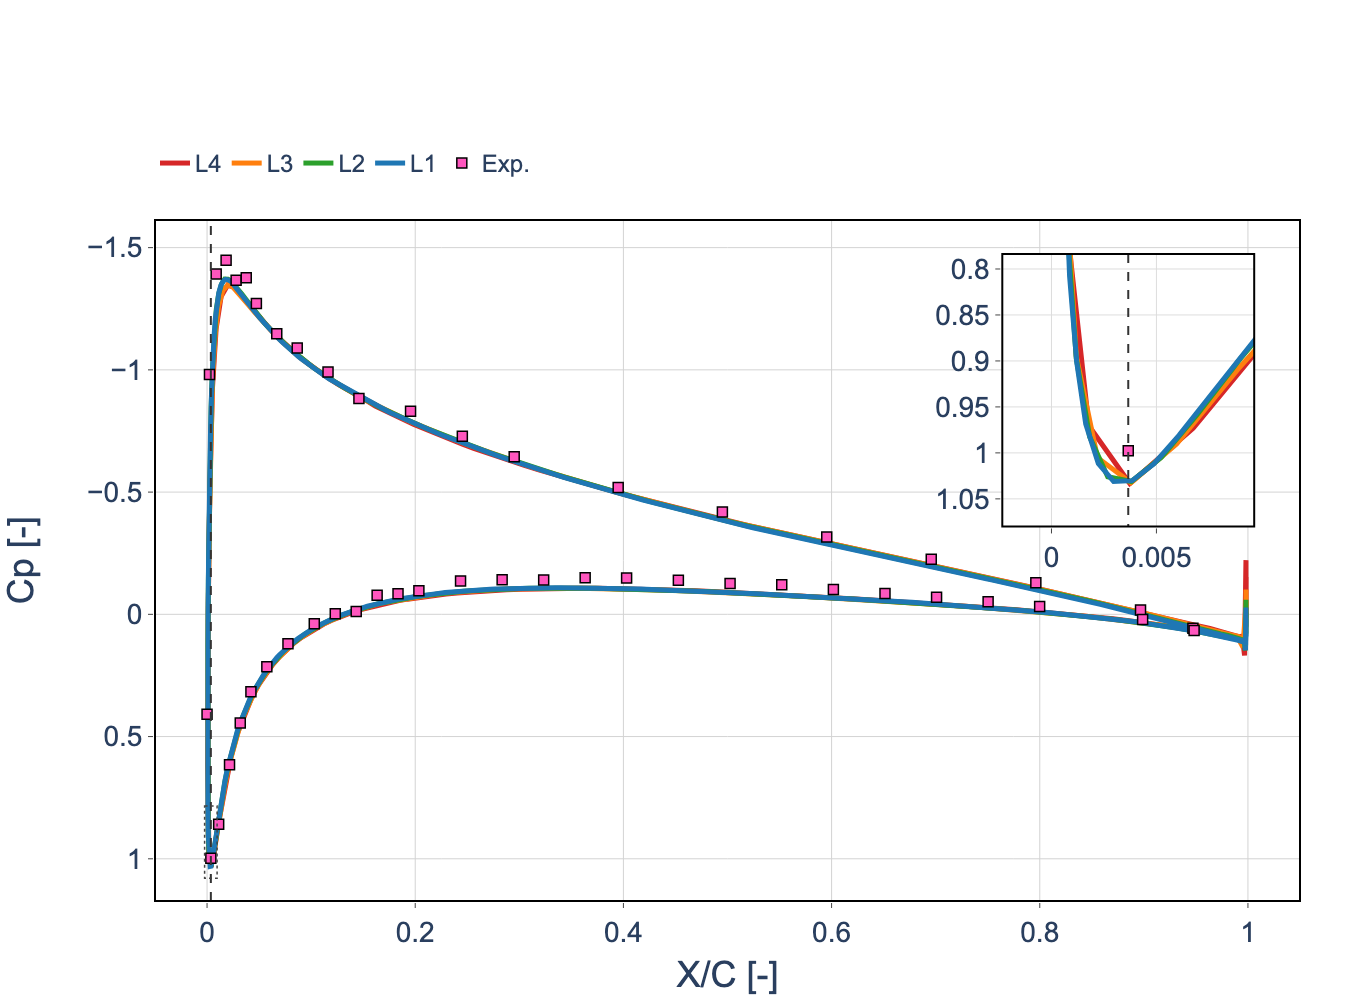
\includegraphics[width=0.84\linewidth]{FIGURES/NACA0012/AERODYNAMIC/tc_naca0012_ae3932_L1_cp_vs_x_slice_0p9144_all_roughness.png}
    \caption{NACA~0012 Level~1 surface-pressure coefficient distribution for condition AE3932.}
    \label{fig:nacaAero}
\end{figure}

Droplet impingement is examined through both spatial and droplet-size refinement. As shown in Fig.~\ref{fig:nacaBins}, increasing the number of droplet bins broadens the impingement region. The peak collection efficiency decreases slightly as the number of bins increases, while the largest differences occur in the impingement limits. This illustrates that convergence of the integrated collected-water mass does not necessarily imply convergence of the local impingement distribution.

\begin{figure}[htb]
    \centering
    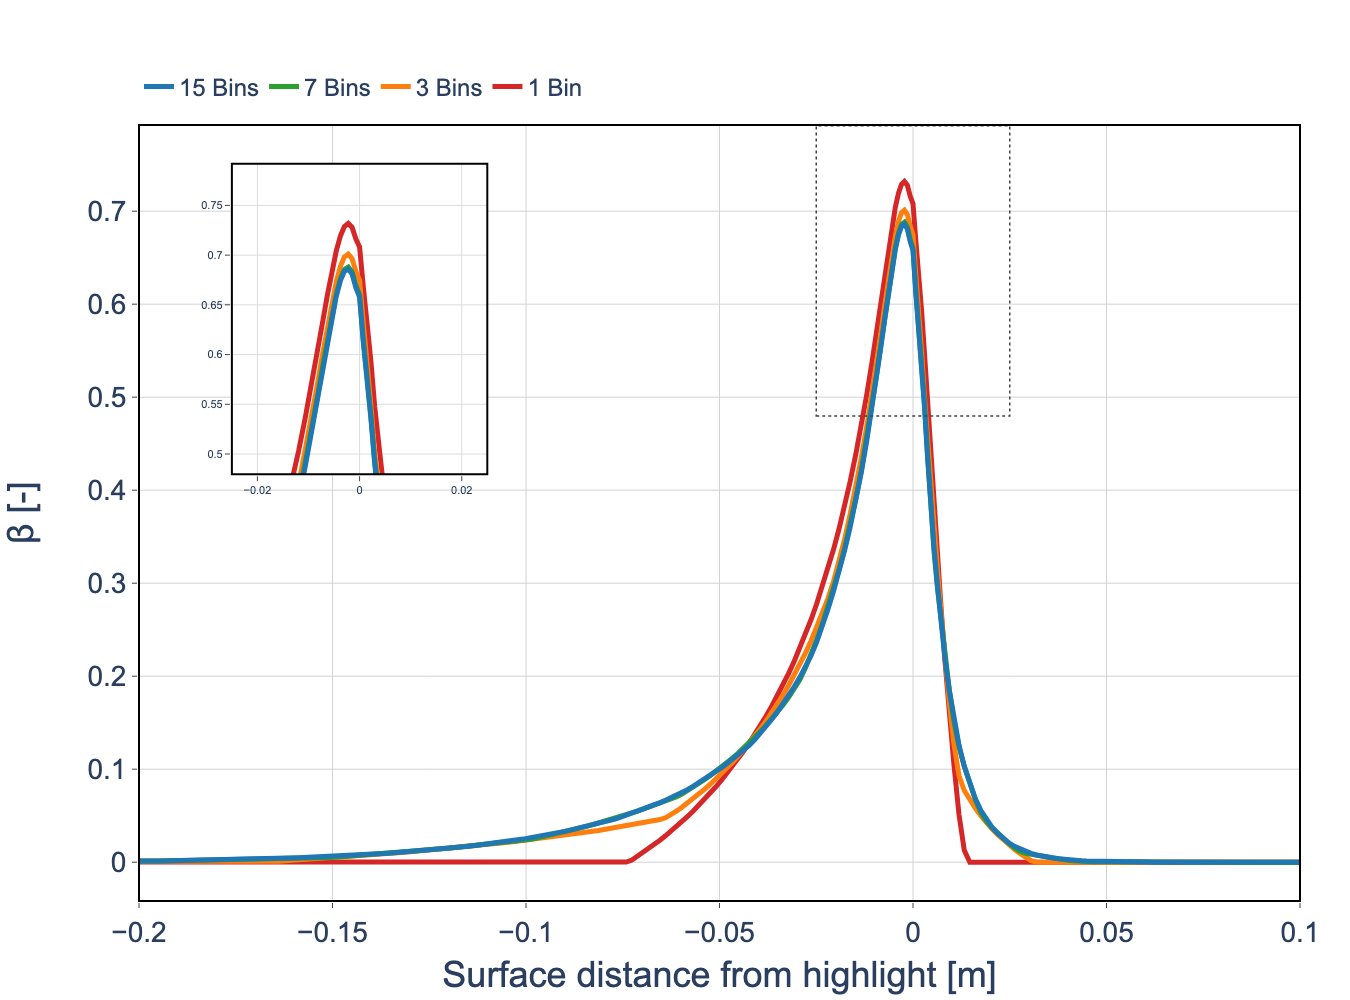
\includegraphics[width=0.86\linewidth]
    {FIGURES/NACA0012/IMPINGEMENT/tc_naca0012_ae3932_beta_bins07_vs_s_slice_0p9144_all_roughness_eulerian_grid_levels.png}
    \caption{Effect of droplet-size discretization on the NACA~0012 collection-efficiency distribution for condition AE3932.}
    \label{fig:nacaBins}
\end{figure}

Complementary Eulerian and Lagrangian calculations provide an independent verification of the impingement solution. On the Level~1 grid, the difference in collected-water mass between the two formulations is less than $1\%$ for both the single-bin and 7-bin distributions. The close agreement is maintained across the workshop grid hierarchy, as shown in Fig.~\ref{fig:eulLag}. Increasing the droplet representation from one to 7-bins increases the predicted collected-water mass by approximately $8\%$, while producing a more pronounced change in the extent of the impingement region.

\begin{figure}[htb]
    \centering
    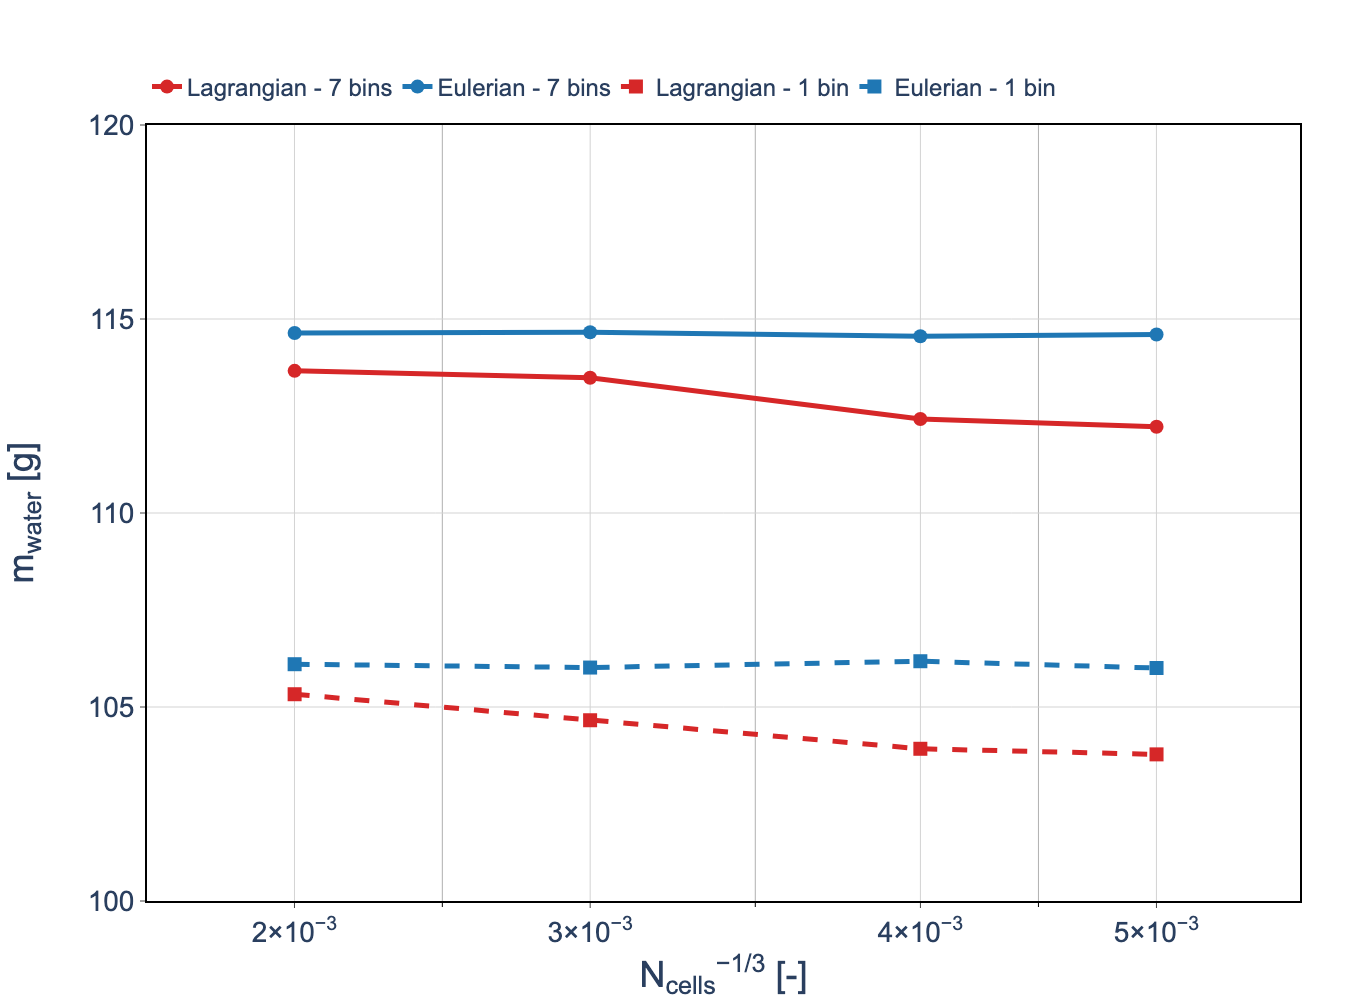
\includegraphics[width=0.86\linewidth]{FIGURES/NACA0012/IMPINGEMENT/tc_naca0012_ae3932_water_mass_vs_n_lagrangian_vs_eulerian_bins01_bins07.png}
    \caption{Eulerian and Lagrangian collected-water mass for NACA~0012 AE3932 using 1- and 7-bin droplet distributions.}
    \label{fig:eulLag}
\end{figure}

Experimentally, the ice mass decreases by approximately $15\%$ between AE3932 and AE3933. The numerical prediction exhibits a substantially smaller reduction of approximately $1.5\%$, indicating insufficient thermodynamic sensitivity to the change in thermal condition. Despite this discrepancy, the single-layer calculations reproduce the experimentally observed change in upper-horn orientation between the two conditions and exhibit limited spatial sensitivity, as shown in Fig.~\ref{fig:nacaIce}.

\begin{figure}[htb]
    \centering
    \begin{minipage}[c]{0.48\linewidth}
        \centering
        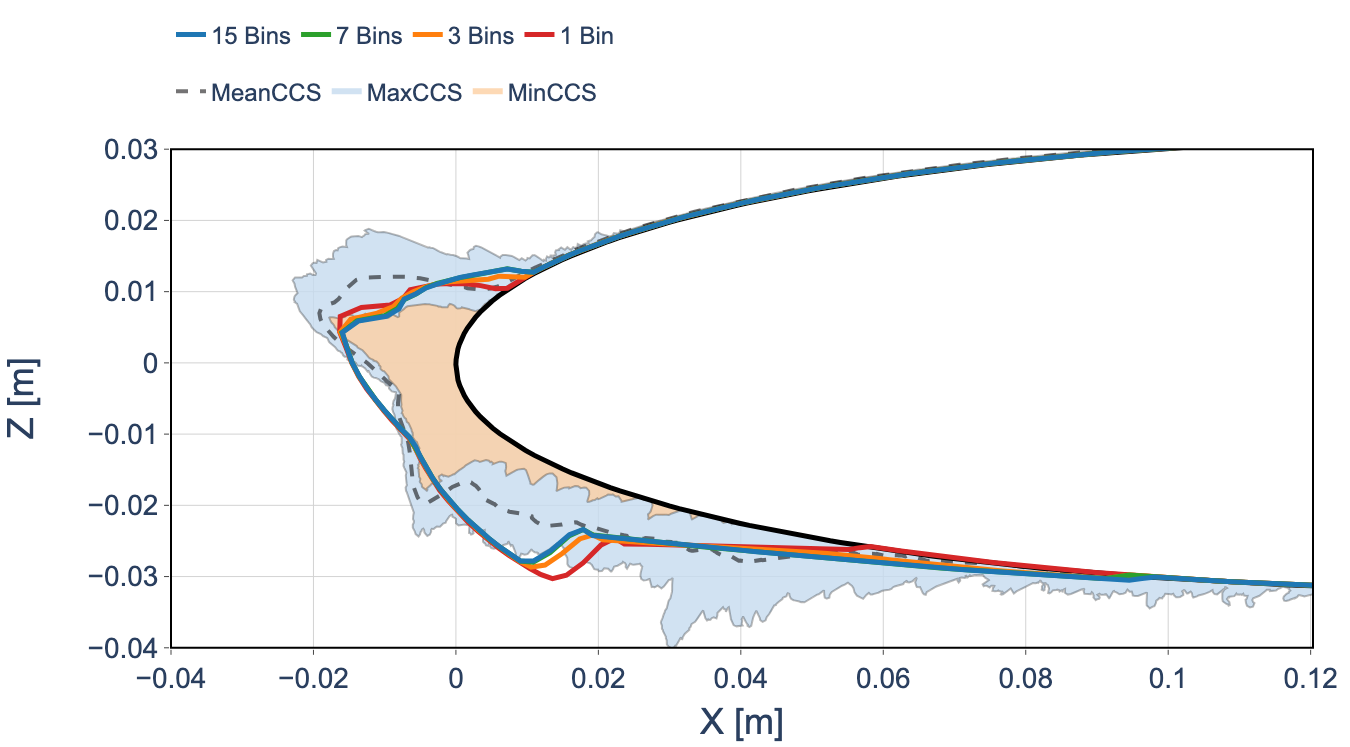
\includegraphics[width=\linewidth]{FIGURES/NACA0012/ICE_SHAPES/tc_naca0012_ae3932_L1_single_layer_ice_shape_slice_0p9144_all_bins.png}

        \small (a) AE3932
    \end{minipage}
    \hfill
    \begin{minipage}[c]{0.48\linewidth}
        \centering
        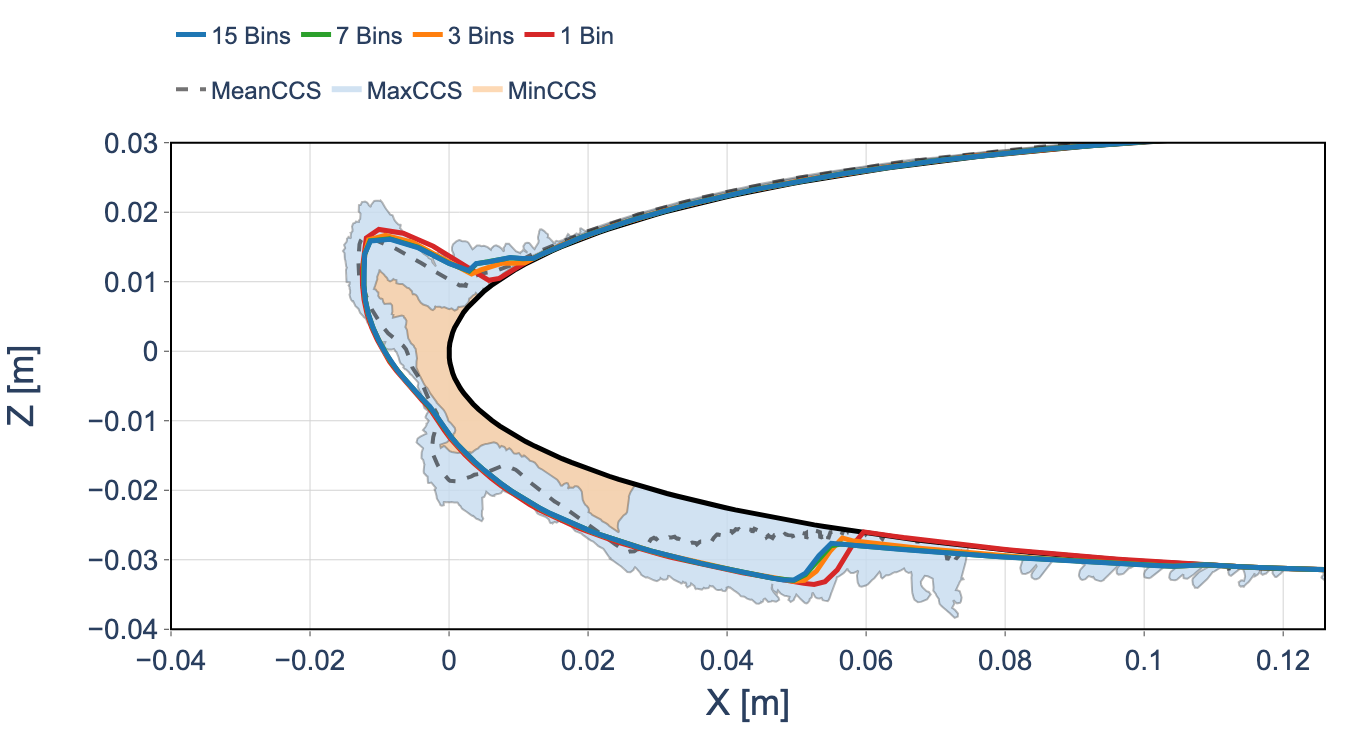
\includegraphics[width=\linewidth]{FIGURES/NACA0012/ICE_SHAPES/tc_naca0012_ae3933_L1_single_layer_ice_shape_slice_0p9144_all_bins.png}

        \small (b) AE3933
    \end{minipage}
    \caption{NACA~0012 Level~1 single-layer ice shapes showing the change in horn morphology between AE3932 and AE3933.}
    \label{fig:nacaIce}
\end{figure}

% ------------------------------------------------------------
% ONERA M6
% ------------------------------------------------------------

\subsection{ONERA~M6}

The ONERA~M6 configuration extends the verification and validation to a fully three-dimensional swept wing. The prescribed grids range from approximately $1.35\times10^5$ cells on Level~4 to $6.92\times10^7$ cells on Level~1. The aerodynamic predictions exhibit systematic spatial convergence. As shown in Fig.~\ref{fig:m6Cp}, the surface-pressure distributions at the midspan slice, $y=0.75$~m, are nearly superimposed over most of the chord, with the largest grid sensitivity concentrated near the leading-edge suction peak. The three finest grid levels show particularly close agreement.

\begin{figure}[htb]
    \centering
    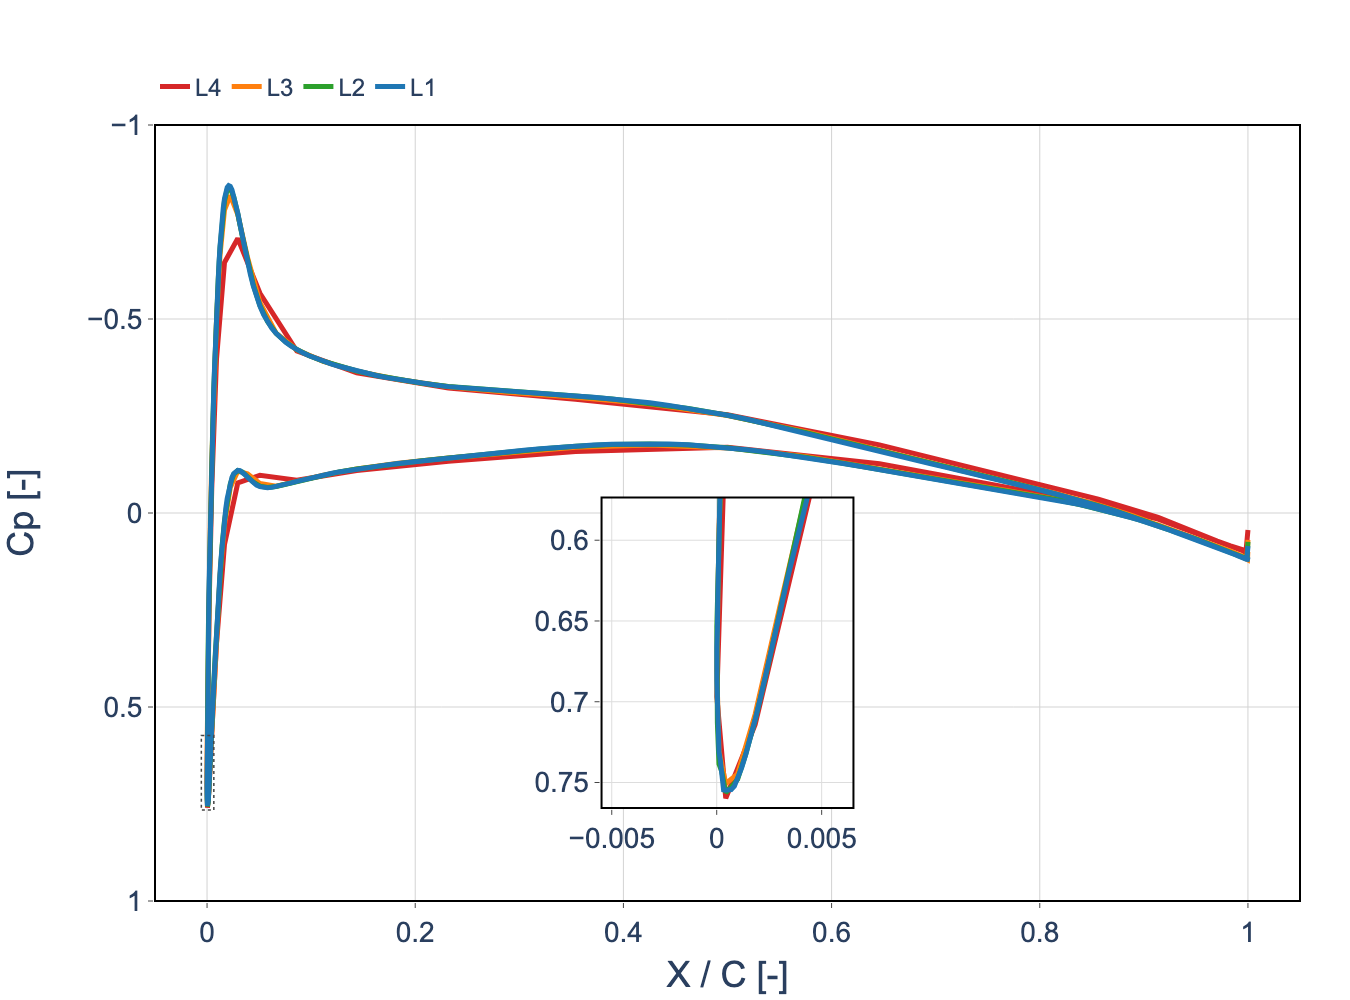
\includegraphics[width=0.86\linewidth]
    {FIGURES/ONERAM6/AERODYNAMIC/tc_oneram6_L1_cp_vs_x_slice_0p75_roughness_1mm.png}
    \caption{ONERA~M6 surface-pressure coefficient distributions across the prescribed grid hierarchy at the midspan slice, $y=0.75$~m.}
    \label{fig:m6Cp}
\end{figure}

As for the NACA~0012 configuration, complementary Eulerian and Lagrangian droplet calculations produce closely matching collection-efficiency distributions for the ONERA~M6. Figure~\ref{fig:m6EulLag} shows the comparison at the intermediate spanwise station, $y=0.75$~m, on the Level~1 grid. Both formulations predict comparable peak collection efficiencies and impingement limits, providing an independent verification of the Eulerian impingement solution for a three-dimensional swept-wing configuration.

\begin{figure}[htb]
    \centering
    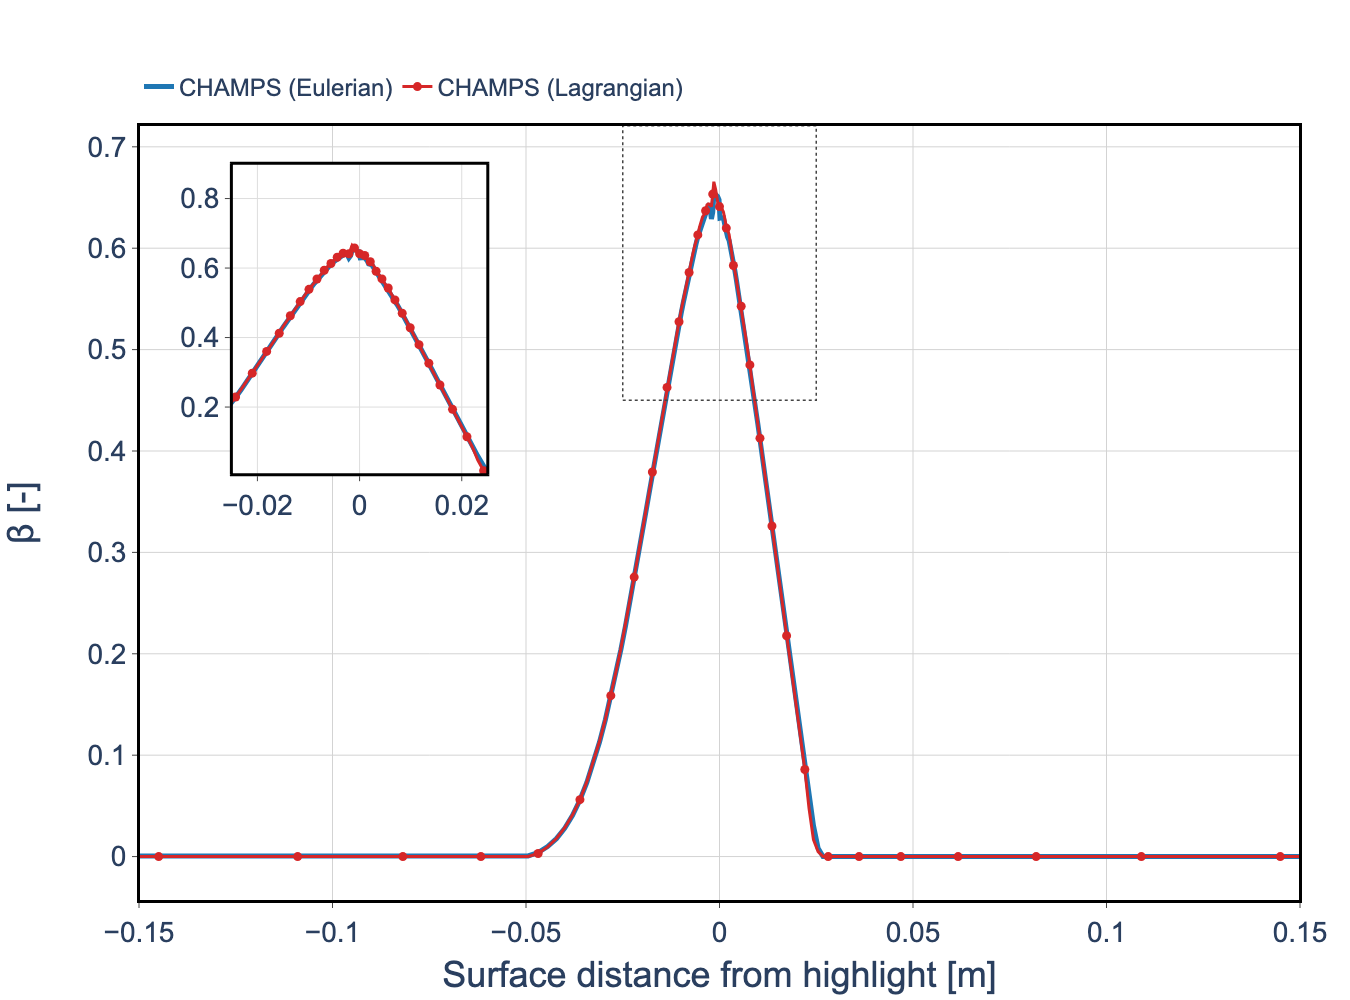
\includegraphics[width=0.86\linewidth]{FIGURES/ONERAM6/IMPINGEMENT/tc_oneram6_L1_beta_bins01_vs_s_slice_0p75_roughness_1mm.png}
    \caption{Eulerian and Lagrangian collection-efficiency distributions for the ONERA~M6 on the Level~1 grid at $y=0.75$~m using the single-bin droplet distribution.}
    \label{fig:m6EulLag}
\end{figure}

Single-layer ice shapes exhibit relatively limited sensitivity over the finer workshop grids. Multilayer calculations using the continuous level-set framework produce pronounced three-dimensional horn structures and spanwise variations, as illustrated in Fig.~\ref{fig:m6Ice}.

\begin{figure}[htb]
    \centering
    \begin{minipage}[c]{0.48\linewidth}
        \centering
        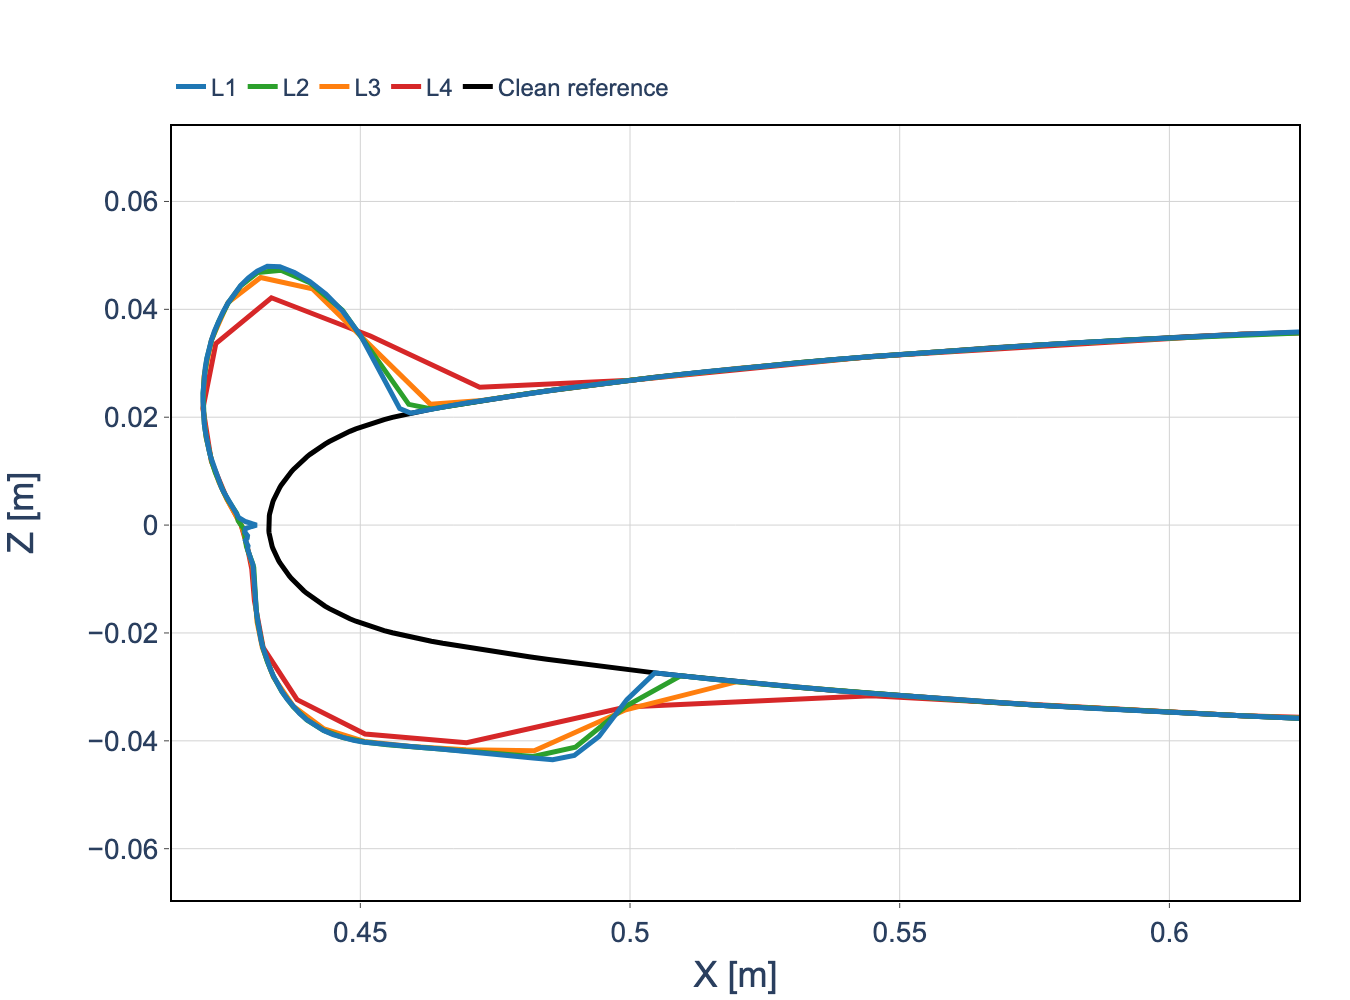
\includegraphics[width=\linewidth]{FIGURES/ONERAM6/ICE_SHAPES/tc_oneram6_L1_single_layer_ice_shape_slice_0p75_bins07_roughness_1mm.png}

        \small (a) Single layer
    \end{minipage}
    \hfill
    \begin{minipage}[c]{0.48\linewidth}
        \centering
        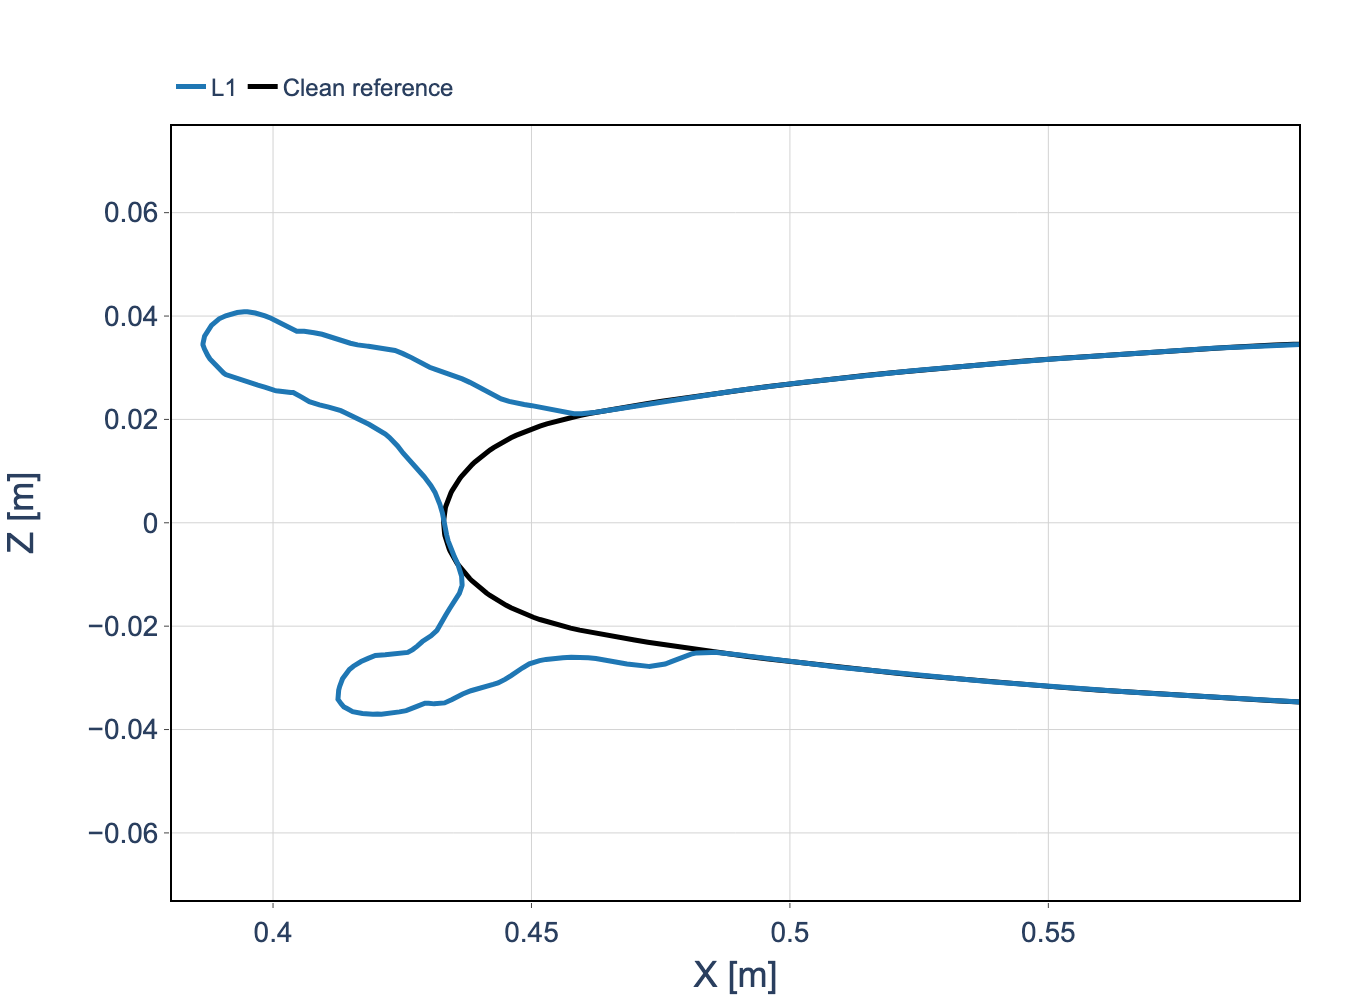
\includegraphics[width=\linewidth]{FIGURES/ONERAM6/ICE_SHAPES/tc_oneram6_L1_multilayer_ice_shape_slice_0p75_bins07_roughness_1mm.png}

        \small (b) Multilayer
    \end{minipage}
    \caption{ONERA~M6 Level~1 single-layer and multilayer ice-shape predictions at $y=0.75$~m.}
    \label{fig:m6Ice}
\end{figure}

The results from both configurations demonstrate the importance of considering local and integrated quantities separately. Integrated water or ice mass may exhibit limited sensitivity while local impingement limits or ice morphology remain noticeably different.

% ============================================================
% EXPECTED RESULTS
% ============================================================

\section{Expected Results}

The completed study will provide the full Polytechnique Montr\'{e}al IPW3 verification and validation results for the NACA~0012 and ONERA~M6 configurations. The final analysis will also investigate multilayer geometry evolution, including the influence of evolving surface normals, more advanced spatially and temporally varying roughness models, and ice-density modeling. Comparisons with experimental measurements and IPW3 participant data will be used to determine how these modeling choices influence integrated ice mass, horn orientation, and three-dimensional ice morphology.

\bibliographystyle{ieeetr} % closest to SAE
\bibliography{references}

\section{Contact Information}
Mohamad Karim Zayni\newline
mohamad-karim.zayni@polymtl.ca

% ============================================================
% ACKNOWLEDGEMENTS
% ============================================================

\section{Acknowledgements}

This work was supported in part by the Canada Research Chairs Program,
the Natural Sciences and Engineering Research Council of Canada (NSERC),
and the Digital Research Alliance of Canada. The authors gratefully
acknowledge the organizers and participants of the Third AIAA Ice
Prediction Workshop for providing the computational grids, experimental
data, and code-to-code comparison data used in this study.


% ============================================================
% DEFINITIONS, ACRONYMS, AND ABBREVIATIONS
% ============================================================

\section{Definitions, Acronyms, Abbreviations}

\begin{table}[h]
\centering
\begin{tabular}{L{0.12\textwidth} L{0.35\textwidth}}
\textbf{CFD}    & Computational Fluid Dynamics \\
\textbf{CHAMPS} & Computational Hierarchical Advanced Multiphysics Solver \\
\textbf{IPW}    & AIAA Ice Prediction Workshop \\
\textbf{IPW3}   & Third AIAA Ice Prediction Workshop \\
\textbf{MVD}    & Median Volumetric Diameter \\
\textbf{RANS}   & Reynolds-Averaged Navier--Stokes \\
\end{tabular}
\end{table}


% ------------------------------------------------------------
% General symbols
% ------------------------------------------------------------

\textbf{General symbols}

\begin{table}[h]
\centering
\begin{tabular}{L{0.08\textwidth} L{0.29\textwidth} L{0.08\textwidth}}
$C_D$   & Drag coefficient             & $[-]$ \\
$C_L$   & Lift coefficient             & $[-]$ \\
$C_{MY}$ & Pitching-moment coefficient & $[-]$ \\
$C_p$   & Pressure coefficient         & $[-]$ \\
$y$     & Spanwise coordinate          & $[\mathrm{m}]$ \\
\end{tabular}
\end{table}


% ------------------------------------------------------------
% Greek symbols
% ------------------------------------------------------------

\textbf{Greek symbols}

\begin{table}[h]
\centering
\begin{tabular}{L{0.08\textwidth} L{0.29\textwidth} L{0.08\textwidth}}
$\beta$ & Droplet collection efficiency & $[-]$ \\
$\phi$  & Level-set signed-distance function & $[\mathrm{m}]$ \\
\end{tabular}
\end{table}


\end{document}
